\documentclass[11pt]{article}
\usepackage[margin=2.3cm]{geometry}
\usepackage[T1]{fontenc}
\usepackage{lmodern}
\usepackage{amsmath,amssymb}
\usepackage{booktabs}
\usepackage{graphicx}
\usepackage{xcolor}
\usepackage{listings}
\usepackage{float}
\usepackage{caption}
\usepackage{fancyhdr}
\usepackage[hidelinks]{hyperref}

\pagestyle{fancy}
\fancyhf{}
\lhead{COMP7103 Assignment 1}
\rhead{Data Mining}
\cfoot{\thepage}
\setlength{\headheight}{14pt}

\lstset{
  language=Python,
  basicstyle=\ttfamily\footnotesize,
  breaklines=true,
  frame=single,
  columns=fullflexible,
  keepspaces=true,
  showstringspaces=false,
  numbers=left,
  numberstyle=\tiny\color{black!60},
  numbersep=6pt,
  xleftmargin=1.6em,
  aboveskip=0.6em,
  belowskip=0.4em
}

\captionsetup{font=small,skip=6pt}
\setkeys{Gin}{keepaspectratio}

\title{\textbf{COMP7103 Assignment 1}\\[0.4em]
\large Data Mining}
\author{Name: \underline{\hspace{5.5cm}} \quad University No.: \underline{\hspace{4.2cm}}}
\date{Due 6 November 2026, 11:59\,pm (Hong Kong)}

\begin{document}
\maketitle
\thispagestyle{fancy}

\noindent
Norms used throughout are the standard $L_p$ norms. For a vector $V=(v_1,\ldots,v_d)$,
\[
\|V\|_1=\sum_{i=1}^{d}|v_i|,\qquad
\|V\|_2=\sqrt{\sum_{i=1}^{d}v_i^2},\qquad
\|V\|_\infty=\max_i|v_i|.
\]
The absolute values are required for $\|\cdot\|_1$ and $\|\cdot\|_\infty$; otherwise these would not be norms. Cosine similarity and information gain use $\log_2$. Entropies and gains below are reported to 6 decimal places. A gain is compared with the pre-pruning threshold $0.15$ before that rounding.

\tableofcontents
\vspace{0.5em}

%----------------------------------------------------------------------
\section{Question 1: Similarity measures}

Let the term order be (borrow, film, good, great, know, movie, part, think). The five term-frequency vectors are
\begin{align*}
R_1 &= (0,0,2,2,1,5,0,2),\\
R_2 &= (0,5,0,1,3,4,2,1),\\
R_3 &= (3,0,2,0,0,10,2,2),\\
R_4 &= (0,3,0,0,1,4,0,0),\\
R_5 &= (0,1,2,2,0,4,0,0).
\end{align*}
Cosine similarity is
\[
\cos(A,B)=\frac{A\cdot B}{\|A\|_2\,\|B\|_2}.
\]

\subsection*{1(a) Most similar reviews under term frequency}

Squared lengths, obtained by summing the squared components:
\[
\begin{aligned}
\|R_1\|_2^2&=38, & \|R_2\|_2^2&=56, & \|R_3\|_2^2&=121,\\
\|R_4\|_2^2&=26, & \|R_5\|_2^2&=25.
\end{aligned}
\]
So $\|R_3\|_2=11$ and $\|R_5\|_2=5$. The ten pairwise dot products and cosine similarities are:

\begin{center}
\small
\begin{tabular}{lrrrr}
\toprule
Pair & Dot product & $\|R_a\|_2^2$ & $\|R_b\|_2^2$ & Cosine \\
\midrule
$R_1,R_5$ & 28 & 38 & 25 & \textbf{0.908440} \\
$R_2,R_4$ & 34 & 56 & 26 & 0.891042 \\
$R_1,R_3$ & 58 & 38 & 121 & 0.855349 \\
$R_3,R_5$ & 44 & 121 & 25 & 0.800000 \\
$R_4,R_5$ & 19 & 26 & 25 & 0.745241 \\
$R_3,R_4$ & 40 & 121 & 26 & 0.713150 \\
$R_1,R_4$ & 21 & 38 & 26 & 0.668099 \\
$R_2,R_5$ & 23 & 56 & 25 & 0.614701 \\
$R_1,R_2$ & 27 & 38 & 56 & 0.585299 \\
$R_2,R_3$ & 46 & 56 & 121 & 0.558819 \\
\bottomrule
\end{tabular}
\end{center}

The largest value is $\cos(R_1,R_5)$. Its dot product expands as
\[
R_1\cdot R_5 = 2\cdot 2 + 2\cdot 2 + 5\cdot 4 = 4+4+20 = 28,
\]
and
\[
\cos(R_1,R_5)=\frac{28}{\sqrt{38}\cdot 5}=\frac{28}{5\sqrt{38}}=0.908440.
\]
The next largest value is $\cos(R_2,R_4)=0.891042$, so the maximum is unique.

\textbf{Answer.} The most similar pair under term frequency is reviews 1 and 5, with cosine similarity $0.908440$.

\subsection*{1(b) TF--IDF and the most similar pair}

There are $|D|=5$ reviews. Term frequency is the raw count. Document frequencies and
$\mathrm{idf}(t)=\log_2(|D|/|D_t|)$ are:

\begin{center}
\small
\begin{tabular}{lccc}
\toprule
Term & $|D_t|$ & idf & value \\
\midrule
borrow & 1 & $\log_2 5$ & 2.321928 \\
film, good, great, know, think & 3 & $\log_2(5/3)$ & 0.736966 \\
part & 2 & $\log_2(5/2)$ & 1.321928 \\
movie & 5 & $\log_2 1$ & 0 \\
\bottomrule
\end{tabular}
\end{center}

\noindent Movie occurs in every review, so its idf is $\log_2 1=0$ and it drops out of every TF--IDF vector. Multiplying each raw count by the idf of its term gives
\begin{align*}
R_1 &= (0,\ 0,\ 1.473931,\ 1.473931,\ 0.736966,\ 0,\ 0,\ 1.473931),\\
R_2 &= (0,\ 3.684828,\ 0,\ 0.736966,\ 2.210897,\ 0,\ 2.643856,\ 0.736966),\\
R_3 &= (6.965784,\ 0,\ 1.473931,\ 0,\ 0,\ 0,\ 2.643856,\ 1.473931),\\
R_4 &= (0,\ 2.210897,\ 0,\ 0,\ 0.736966,\ 0,\ 0,\ 0),\\
R_5 &= (0,\ 0.736966,\ 1.473931,\ 1.473931,\ 0,\ 0,\ 0,\ 0).
\end{align*}
(Each displayed component is $\mathrm{tf}\times\mathrm{idf}$ rounded to 6 decimal places. The cosines below use the unrounded products.)

\begin{center}
\small
\begin{tabular}{lrrr}
\toprule
Pair & Dot product & Cosine \\
\midrule
$R_2,R_4$ & 9.776129 & \textbf{0.814237} \\
$R_1,R_5$ & 4.344946 & 0.739600 \\
$R_2,R_5$ & 3.801828 & 0.333776 \\
$R_4,R_5$ & 1.629355 & 0.316228 \\
$R_1,R_2$ & 3.801828 & 0.277719 \\
$R_1,R_3$ & 4.344946 & 0.211353 \\
$R_2,R_3$ & 8.076212 & 0.202620 \\
$R_3,R_5$ & 2.172473 & 0.127007 \\
$R_1,R_4$ & 0.543118 & 0.087706 \\
$R_3,R_4$ & 0 & 0.000000 \\
\bottomrule
\end{tabular}
\end{center}

For the winning pair, write $\alpha=\log_2(5/3)$. The only nonzero contributions to $R_2\cdot R_4$ are film and know:
\[
R_2\cdot R_4 = (5\alpha)(3\alpha) + (3\alpha)(1\alpha) = 18\alpha^2 = 9.776129.
\]
The Euclidean norms are $\|R_2\|_2=5.151916$ and $\|R_4\|_2=2.330490$, so
\[
\cos(R_2,R_4)=\frac{9.776129}{5.151916\times 2.330490}=0.814237.
\]
The runner-up is $\cos(R_1,R_5)=0.739600$. Reweighting by idf changes the most similar pair: ``movie'' no longer contributes, and reviews 2 and 4 share the comparatively rare term ``film''.

\textbf{Answer.} The most similar pair under TF--IDF is reviews 2 and 4, with cosine similarity $0.814237$.

%----------------------------------------------------------------------
\section{Question 2: Metric axioms}

A function $d$ is a metric when it satisfies all three of the following, for every data object $p,q,r$.
\begin{itemize}
  \item \textbf{Positivity.} $d(p,q)\ge 0$, and $d(p,q)=0$ if and only if $p=q$. Objects are identified by their position and orientation, so $p=q$ means $P_p=P_q$ and $\Theta_p=\Theta_q$.
  \item \textbf{Symmetry.} $d(p,q)=d(q,p)$.
  \item \textbf{Triangle inequality.} $d(p,r)\le d(p,q)+d(q,r)$.
\end{itemize}
Positions below are in millimetres. Orientation components are integers in $[0,360)$. The difference $\Theta_p-\Theta_q$ is ordinary vector subtraction, as specified by the $L_p$ norm of that difference.

\subsection*{2(a) $d_1(p,q)=\min(\|P_p-P_q\|_1,\|\Theta_p-\Theta_q\|_1)$}

\textbf{Positivity fails.} Take
\[
p:\ P=(0,0,0),\ \Theta=(0,0,0),
\qquad
q:\ P=(0,0,0),\ \Theta=(10,0,0).
\]
Then $p\neq q$, but $\|P_p-P_q\|_1=0$ and $\|\Theta_p-\Theta_q\|_1=10$, so $d_1(p,q)=\min(0,10)=0$.

\textbf{Symmetry holds.} For any vector $V$, $\|V\|_1=\|-V\|_1$. Therefore both arguments of the minimum are unchanged when $p$ and $q$ are swapped, and so is the minimum.

\textbf{Triangle inequality fails.} Take
\begin{align*}
a&:\ P=(0,0,0),\ \Theta=(0,0,0),\\
b&:\ P=(5,0,0),\ \Theta=(0,0,0),\\
c&:\ P=(5,0,0),\ \Theta=(5,0,0).
\end{align*}
Then
\begin{align*}
d_1(a,b)&=\min(5,0)=0,\\
d_1(b,c)&=\min(0,5)=0,\\
d_1(a,c)&=\min(5,5)=5.
\end{align*}
Since $5\not\le 0+0$, the triangle inequality fails.

\subsection*{2(b) $d_2(p,q)=\|P_p-P_q\|_2+\|\Theta_p-\Theta_q\|_\infty$}

Write $d_P(p,q)=\|P_p-P_q\|_2$ and $d_\Theta(p,q)=\|\Theta_p-\Theta_q\|_\infty$. Euclidean distance and $L_\infty$ distance are both metrics, and $d_2=d_P+d_\Theta$.

\textbf{Positivity holds.} A sum of nonnegative numbers is nonnegative. The sum is zero only when both terms are zero, hence only when $P_p=P_q$ and $\Theta_p=\Theta_q$.

\textbf{Symmetry holds.} Both $d_P$ and $d_\Theta$ are symmetric, so their sum is symmetric.

\textbf{Triangle inequality holds.} For any $a,b,c$,
\[
d_P(a,c)\le d_P(a,b)+d_P(b,c), \qquad d_\Theta(a,c)\le d_\Theta(a,b)+d_\Theta(b,c).
\]
Adding these two inequalities gives $d_2(a,c)\le d_2(a,b)+d_2(b,c)$.

Thus $d_2$ satisfies all three axioms.

\subsection*{2(c) $d_3(p,q)=(\|P_p-P_q\|_2)^2+\|\Theta_p-\Theta_q\|_1$}

\textbf{Positivity holds.} Both terms are nonnegative, so $d_3(p,q)\ge 0$. The square of an $L_2$ norm is zero exactly when the vector is zero, and an $L_1$ norm is zero exactly when its vector is zero. Hence $d_3(p,q)=0$ exactly when the position vectors agree and the orientation vectors agree. Also $d_3(p,p)=0$.

\textbf{Symmetry holds.} Replacing a difference by its negative does not change either norm, and squaring does not change that fact.

\textbf{Triangle inequality fails.} Use three positions on a line and identical orientations, so the orientation term is zero:
\begin{align*}
a&:\ P=(0,0,0),\ \Theta=(0,0,0),\\
b&:\ P=(1,0,0),\ \Theta=(0,0,0),\\
c&:\ P=(2,0,0),\ \Theta=(0,0,0).
\end{align*}
Then $d_3(a,b)=1^2=1$, $d_3(b,c)=1$, and $d_3(a,c)=2^2=4$. Since $4\not\le 1+1$, the triangle inequality fails. Setting the orientations equal isolates the squared Euclidean distance, which is what breaks the axiom; the added orientation term does not repair it.

\subsection*{2(d) $d_4(p,q)=\|P_p\|_2-\|P_q\|_2+\|\Theta_p\|_2-\|\Theta_q\|_2$}

Define $f(x)=\|P_x\|_2+\|\Theta_x\|_2$. Then $d_4(p,q)=f(p)-f(q)$.

\textbf{Positivity fails.} Take
\[
p:\ P=(0,0,0),\ \Theta=(0,0,0),
\qquad
q:\ P=(3,4,0),\ \Theta=(0,0,0).
\]
Then $f(p)=0$, $f(q)=\|(3,4,0)\|_2=5$, and $d_4(p,q)=-5<0$.

\textbf{Symmetry fails.} For the same pair, $d_4(q,p)=5\neq -5=d_4(p,q)$.

\textbf{Triangle inequality holds.} For every triple $p,q,r$,
\begin{align*}
d_4(p,q)+d_4(q,r)
&= \bigl(f(p)-f(q)\bigr)+\bigl(f(q)-f(r)\bigr)\\
&= f(p)-f(r)\\
&= d_4(p,r).
\end{align*}
The two sides are equal, so $d_4(p,r)\le d_4(p,q)+d_4(q,r)$ holds for every triple, including triples that produce a negative value.

%----------------------------------------------------------------------
\section{Question 3: Classification}

Entropy of a set $D$ with class proportions $p_c$ is $H(D)=-\sum_c p_c\log_2 p_c$, and a binary split into $L$ and $R$ has information gain
\[
\mathrm{Gain}(D)=H(D)-\frac{|L|}{|D|}H(L)-\frac{|R|}{|D|}H(R).
\]
A node is split only when it contains at least 8 training instances and its best binary split has gain at least $0.15$. Otherwise it becomes a leaf labelled with its majority class. Every leaf below has a unique majority, so no tie-break is required.

Smoking is nominal, so a binary split is a partition of its values, not a numeric threshold. Age is numeric. Each candidate threshold is the midpoint between two successive distinct ages present in the node; every instance with a given age then falls entirely on one side.

\subsection*{The tree}

\begin{quote}
Smoking $\in\{1,3\}$?\\
\quad yes, and Age $\le 62.5$: predict \textbf{HC} \quad (8 instances; best gain $0.143156<0.15$)\\
\quad yes, and Age $> 62.5$: predict \textbf{COPD} \quad (3 instances)\\
\quad no (Smoking $=2$): predict \textbf{Asthma} \quad (7 instances)
\end{quote}

On the six test records this tree predicts HC, HC, Asthma, HC, COPD, Asthma. None of those predictions matches the true label, so the test accuracy is $0/6=0$. The multi-way gain ratio of Smoking on the training set is $0.179595$. The working is below.

\subsection*{3(a)(i) Induction}

\subsection*{Training distribution}
The training set has 18 instances. Class counts: HC 7, Infected 3, Asthma 5, COPD 3.
\subsection*{Root}

Records 1, 2, 3, 4, 5, 6, 7, 8, 9, 10, 11, 12, 13, 14, 15, 16, 17, 18 ($n=18$). Class counts: HC 7, Infected 3, Asthma 5, COPD 3.
\[ H = -\left(\frac{7}{18}\log_2\frac{7}{18}+\frac{3}{18}\log_2\frac{3}{18}+\frac{5}{18}\log_2\frac{5}{18}+\frac{3}{18}\log_2\frac{3}{18}\right) = 1.904875. \]
Every binary split is evaluated below. For a numeric attribute the threshold is the midpoint between successive distinct values, which puts every instance of one value entirely on one side. For nominal Smoking, each binary split is one partition of the values that actually occur in the node.

\begin{center}
\scriptsize
\begin{tabular}{lrrrrrrr}
\toprule
Split & $|L|$ & $L$ counts & $H(L)$ & $|R|$ & $R$ counts & $H(R)$ & Gain \\
\midrule
Smoking $\in$ {1,3} vs Smoking $\in$ {2} & 11 & 6, 2, 1, 2 & 1.685816 & 7 & 1, 1, 4, 1 & 1.664498 &  \textbf{0.227350} \\
Age $\le$ 59.5 vs Age $>$ 59.5 & 3 & 2, 1, 0, 0 & 0.918296 & 15 & 5, 2, 5, 3 & 1.908613 & 0.161315 \\
Smoking $\in$ {1,2} vs Smoking $\in$ {3} & 14 & 5, 2, 5, 2 & 1.863121 & 4 & 2, 1, 0, 1 & 1.500000 & 0.122448 \\
Age $\le$ 62.5 vs Age $>$ 62.5 & 12 & 6, 2, 3, 1 & 1.729574 & 6 & 1, 1, 2, 2 & 1.918296 & 0.112394 \\
Age $\le$ 58.5 vs Age $>$ 58.5 & 1 & 1, 0, 0, 0 & 0.000000 & 17 & 6, 3, 5, 3 & 1.932805 & 0.079448 \\
Smoking $\in$ {1} vs Smoking $\in$ {2,3} & 7 & 4, 1, 1, 1 & 1.664498 & 11 & 3, 2, 4, 2 & 1.936260 & 0.074300 \\
Age $\le$ 61.5 vs Age $>$ 61.5 & 9 & 4, 1, 3, 1 & 1.752715 & 9 & 3, 2, 2, 2 & 1.974938 & 0.041049 \\
Age $\le$ 60.5 vs Age $>$ 60.5 & 6 & 3, 1, 1, 1 & 1.792481 & 12 & 4, 2, 4, 2 & 1.918296 & 0.028517 \\
\bottomrule
\end{tabular}
\end{center}
Counts are ordered (HC, Infected, Asthma, COPD). The largest gain is in bold.

The best gain is 0.227350, which is at least $0.15$, and the node has at least 8 instances, so the node is split on Smoking $\in$ {1,3} vs Smoking $\in$ {2}.
\[ \mathrm{Gain} = H - \frac{11}{18}H(L) - \frac{7}{18}H(R) = 0.227350. \]
This gain is computed from the unrounded entropies and is the value compared with $0.15$. The entropies in the table are those same quantities rounded to 6 decimal places.

\subsection*{Left child: Smoking $\in \{1,3\}$}

Records 1, 2, 3, 4, 7, 10, 11, 12, 13, 17, 18 ($n=11$). Class counts: HC 6, Infected 2, Asthma 1, COPD 2.
\[ H = -\left(\frac{6}{11}\log_2\frac{6}{11}+\frac{2}{11}\log_2\frac{2}{11}+\frac{1}{11}\log_2\frac{1}{11}+\frac{2}{11}\log_2\frac{2}{11}\right) = 1.685816. \]
Every binary split is evaluated below. For a numeric attribute the threshold is the midpoint between successive distinct values, which puts every instance of one value entirely on one side. For nominal Smoking, each binary split is one partition of the values that actually occur in the node.

\begin{center}
\scriptsize
\begin{tabular}{lrrrrrrr}
\toprule
Split & $|L|$ & $L$ counts & $H(L)$ & $|R|$ & $R$ counts & $H(R)$ & Gain \\
\midrule
Age $\le$ 62.5 vs Age $>$ 62.5 & 8 & 5, 2, 1, 0 & 1.298795 & 3 & 1, 0, 0, 2 & 0.918296 &  \textbf{0.490793} \\
Age $\le$ 61.5 vs Age $>$ 61.5 & 5 & 3, 1, 1, 0 & 1.370951 & 6 & 3, 1, 0, 2 & 1.459148 & 0.266757 \\
Age $\le$ 60.5 vs Age $>$ 60.5 & 4 & 2, 1, 1, 0 & 1.500000 & 7 & 4, 1, 0, 2 & 1.378783 & 0.262953 \\
Age $\le$ 59.5 vs Age $>$ 59.5 & 3 & 2, 1, 0, 0 & 0.918296 & 8 & 4, 1, 1, 2 & 1.750000 & 0.162644 \\
Age $\le$ 58.5 vs Age $>$ 58.5 & 1 & 1, 0, 0, 0 & 0.000000 & 10 & 5, 2, 1, 2 & 1.760964 & 0.084939 \\
Smoking $\in$ {1} vs Smoking $\in$ {3} & 7 & 4, 1, 1, 1 & 1.664498 & 4 & 2, 1, 0, 1 & 1.500000 & 0.081135 \\
\bottomrule
\end{tabular}
\end{center}
Counts are ordered (HC, Infected, Asthma, COPD). The largest gain is in bold.

The best gain is 0.490793, which is at least $0.15$, and the node has at least 8 instances, so the node is split on Age $\le$ 62.5 vs Age $>$ 62.5.
\[ \mathrm{Gain} = H - \frac{8}{11}H(L) - \frac{3}{11}H(R) = 0.490793. \]
This gain is computed from the unrounded entropies and is the value compared with $0.15$. The entropies in the table are those same quantities rounded to 6 decimal places.

\subsection*{Left-left child: Smoking $\in \{1,3\}$ and Age $\le 62.5$}

Records 1, 2, 3, 4, 7, 10, 11, 12 ($n=8$). Class counts: HC 5, Infected 2, Asthma 1.
\[ H = -\left(\frac{5}{8}\log_2\frac{5}{8}+\frac{2}{8}\log_2\frac{2}{8}+\frac{1}{8}\log_2\frac{1}{8}\right) = 1.298795. \]
Every binary split is evaluated below. For a numeric attribute the threshold is the midpoint between successive distinct values, which puts every instance of one value entirely on one side. For nominal Smoking, each binary split is one partition of the values that actually occur in the node.

\begin{center}
\scriptsize
\begin{tabular}{lrrrrrrr}
\toprule
Split & $|L|$ & $L$ counts & $H(L)$ & $|R|$ & $R$ counts & $H(R)$ & Gain \\
\midrule
Age $\le$ 60.5 vs Age $>$ 60.5 & 4 & 2, 1, 1, 0 & 1.500000 & 4 & 3, 1, 0, 0 & 0.811278 & \textbf{0.143156} \\
Smoking $\in$ {1} vs Smoking $\in$ {3} & 6 & 4, 1, 1, 0 & 1.251629 & 2 & 1, 1, 0, 0 & 1.000000 & 0.110073 \\
Age $\le$ 59.5 vs Age $>$ 59.5 & 3 & 2, 1, 0, 0 & 0.918296 & 5 & 3, 1, 1, 0 & 1.370951 & 0.097590 \\
Age $\le$ 61.5 vs Age $>$ 61.5 & 5 & 3, 1, 1, 0 & 1.370951 & 3 & 2, 1, 0, 0 & 0.918296 & 0.097590 \\
Age $\le$ 58.5 vs Age $>$ 58.5 & 1 & 1, 0, 0, 0 & 0.000000 & 7 & 4, 2, 1, 0 & 1.378783 & 0.092359 \\
\bottomrule
\end{tabular}
\end{center}
Counts are ordered (HC, Infected, Asthma, COPD). The largest gain is in bold.

The best gain is 0.143156, which is less than $0.15$. Pre-pruning stops the split. The leaf label is the majority class HC.

\subsection*{Left-right child: Smoking $\in \{1,3\}$ and Age $> 62.5$}

Records 13, 17, 18 ($n=3$). Class counts: HC 1, COPD 2.
\[ H = -\left(\frac{1}{3}\log_2\frac{1}{3}+\frac{2}{3}\log_2\frac{2}{3}\right) = 0.918296. \]
This node has $n=3<8$, so it is not split. The leaf label is the majority class COPD.

\subsection*{Right child: Smoking $= 2$}

Records 5, 6, 8, 9, 14, 15, 16 ($n=7$). Class counts: HC 1, Infected 1, Asthma 4, COPD 1.
\[ H = -\left(\frac{1}{7}\log_2\frac{1}{7}+\frac{1}{7}\log_2\frac{1}{7}+\frac{4}{7}\log_2\frac{4}{7}+\frac{1}{7}\log_2\frac{1}{7}\right) = 1.664498. \]
This node has $n=7<8$, so it is not split. The leaf label is the majority class Asthma.


\subsection*{3(a)(ii) Test evaluation}

\begin{center}
\small
\begin{tabular}{rcccll}
\toprule
Record & Age & Smoking & Actual & Path & Predicted \\
\midrule
19 & 58 & 1 & Infected & $\{1,3\}$, then Age $\le 62.5$ & HC \\
20 & 58 & 3 & Asthma & $\{1,3\}$, then Age $\le 62.5$ & HC \\
21 & 60 & 2 & COPD & Smoking $=2$ & Asthma \\
22 & 62 & 3 & COPD & $\{1,3\}$, then Age $\le 62.5$ & HC \\
23 & 63 & 1 & Asthma & $\{1,3\}$, then Age $>62.5$ & COPD \\
24 & 63 & 2 & HC & Smoking $=2$ & Asthma \\
\bottomrule
\end{tabular}
\end{center}

Record 22 has Age $62$, and $62\le 62.5$, so it follows the HC leaf rather than the COPD leaf. With rows as the actual class and columns as the predicted class, in the order HC, Infected, Asthma, COPD:

\begin{center}
\begin{tabular}{lcccc}
\toprule
Actual $\backslash$ Predicted & HC & Infected & Asthma & COPD \\
\midrule
HC & 0 & 0 & 1 & 0 \\
Infected & 1 & 0 & 0 & 0 \\
Asthma & 1 & 0 & 0 & 1 \\
COPD & 1 & 0 & 1 & 0 \\
\bottomrule
\end{tabular}
\end{center}

No diagonal entry is positive, so
\[
\mathrm{Accuracy}=\frac{0}{6}=0.
\]

\subsection*{Gain ratio of the multi-way Smoking split}

This calculation is separate from the tree. It uses one branch for each value of Smoking on the full training set.
The parent entropy is the root entropy above, $H(D)=1.904875$.
Smoking $= 1$ ($n=7$): HC 4, Infected 1, Asthma 1, COPD 1.

\[ H = -\left(\frac{4}{7}\log_2\frac{4}{7}+\frac{1}{7}\log_2\frac{1}{7}+\frac{1}{7}\log_2\frac{1}{7}+\frac{1}{7}\log_2\frac{1}{7}\right) = 1.664498. \]

Smoking $= 2$ ($n=7$): HC 1, Infected 1, Asthma 4, COPD 1.

\[ H = -\left(\frac{1}{7}\log_2\frac{1}{7}+\frac{1}{7}\log_2\frac{1}{7}+\frac{4}{7}\log_2\frac{4}{7}+\frac{1}{7}\log_2\frac{1}{7}\right) = 1.664498. \]

Smoking $= 3$ ($n=4$): HC 2, Infected 1, COPD 1.

\[ H = -\left(\frac{2}{4}\log_2\frac{2}{4}+\frac{1}{4}\log_2\frac{1}{4}+\frac{1}{4}\log_2\frac{1}{4}\right) = 1.500000. \]

\[ \mathrm{Remainder} = \frac{7}{18}\times 1.664498 + \frac{7}{18}\times 1.664498 + \frac{4}{18}\times 1.500000 = 1.627943. \]
\[ \mathrm{Gain} = 1.904875 - 1.627943 = 0.276932. \]
\[ \mathrm{SplitInfo} = -\left(\frac{7}{18}\log_2\frac{7}{18}+\frac{7}{18}\log_2\frac{7}{18}+\frac{4}{18}\log_2\frac{4}{18}\right) = 1.541982. \]
\[ \mathrm{GainRatio} = \frac{0.276932}{1.541982} = 0.179595. \]


\noindent
Smoking $=3$ has counts $(2,1,1)$ on four instances, so its entropy is exactly
\[
-\bigl(\tfrac12\log_2\tfrac12 + \tfrac14\log_2\tfrac14 + \tfrac14\log_2\tfrac14\bigr)
= \tfrac12 + \tfrac12 = 1.5.
\]
Smoking $=1$ and Smoking $=2$ have the same count multiset $\{4,1,1,1\}$, which is why their entropies agree.

\textbf{Answer.} $\mathrm{GainRatio}(\mathrm{Smoking})=0.179595$.

%----------------------------------------------------------------------
\section{Question 4: Classification in Weka}

The source file has 1{,}197 instances. The ARFF relation \texttt{productivity} keeps \texttt{team}, \texttt{smv}, \texttt{over\_time}, \texttt{incentive}, and \texttt{no\_of\_workers} as numeric attributes, using the original numeric tokens. The class
\[
\texttt{productivity}=\begin{cases}
1 & \text{if }\texttt{actual\_productivity}\ge\texttt{targeted\_productivity},\\
0 & \text{otherwise}
\end{cases}
\]
is declared nominal, \texttt{\{0,1\}}. None of these six fields is missing. The label is 1 on 875 instances and 0 on 322. Weka 3.8.6 was run from the Explorer classify pane, with the class set to \texttt{productivity} and the test option set to 10-fold cross-validation. The result text below is that Explorer output.

\subsection*{4(a) ZeroR}

\begin{figure}[H]
\centering
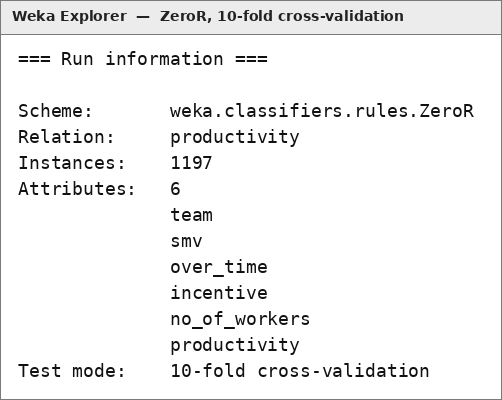
\includegraphics[width=0.86\textwidth]{figures/q4a-run-information.png}
\caption{ZeroR run information. The scheme is \texttt{weka.classifiers.rules.ZeroR} and the test mode is 10-fold cross-validation.}
\end{figure}

\begin{figure}[H]
\centering
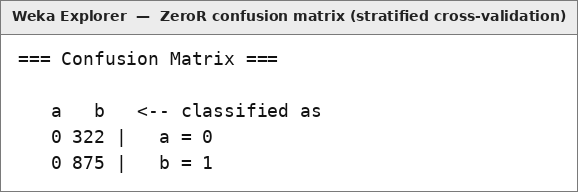
\includegraphics[width=0.92\textwidth]{figures/q4a-confusion-matrix.png}
\caption{Confusion matrix of ZeroR under stratified 10-fold cross-validation. Class \texttt{a} is productivity 0 and class \texttt{b} is productivity 1.}
\end{figure}

\noindent
ZeroR predicts the majority class, which is 1. All 1{,}197 instances are classified as \texttt{b}. The 322 instances of class 0 are errors, so the cross-validated accuracy is $875/1197=73.0994\%$.

\subsection*{4(b) J48 with $C=0.1$}

\begin{figure}[H]
\centering
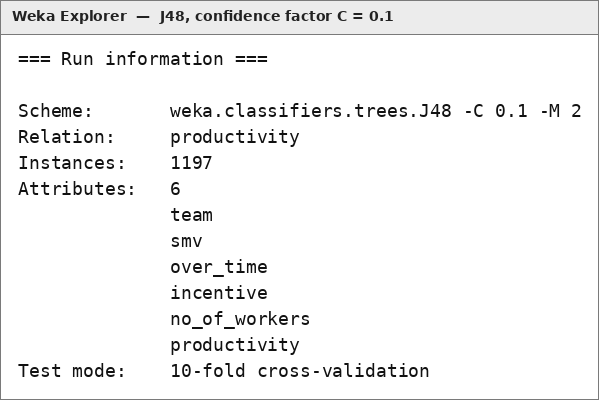
\includegraphics[width=0.92\textwidth]{figures/q4b-run-information.png}
\caption{J48 run information. The confidence factor is $C=0.1$ (\texttt{-C 0.1}); the default minimum leaf size $M=2$ is unchanged. Test mode is 10-fold cross-validation.}
\end{figure}

\begin{figure}[H]
\centering
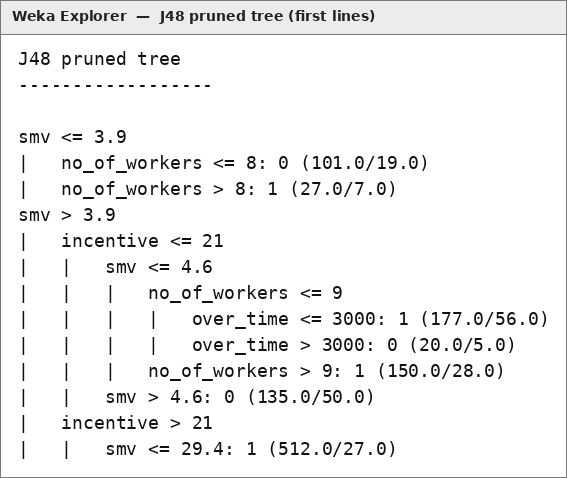
\includegraphics[width=0.86\textwidth]{figures/q4b-tree.png}
\caption{Opening of the J48 pruned tree trained on the full data. The figure contains the tree heading and more than the first ten lines of the tree.}
\end{figure}

\subsection*{4(c) CVParameterSelection on $C$}

\texttt{CVParameterSelection} wraps J48. Its own cross-validation uses 10 folds, and the outer evaluation is also 10-fold cross-validation. The confidence factor $C$ is searched at 16 values from $0.05$ to $0.5$ inclusive. Weka spaces those values by $(0.5-0.05)/(16-1)=0.03$, namely
\[
0.05,0.08,0.11,0.14,\ldots,0.47,0.50.
\]
The initial J48 options after \texttt{--} are the defaults (\texttt{-C 0.25 -M 2}); $C$ is then replaced by the searched value. In the run-information figure the long scheme line is wrapped after \texttt{-S 1}. No tokens were removed.

\begin{figure}[H]
\centering
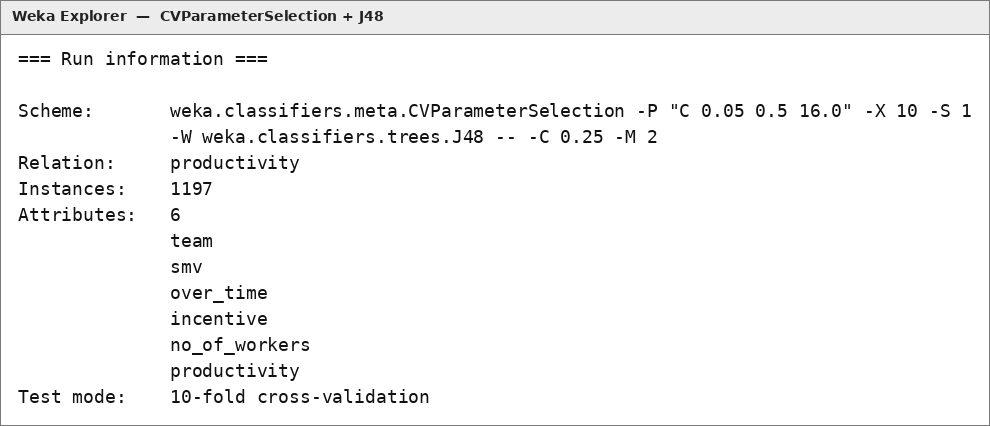
\includegraphics[width=\textwidth]{figures/q4c-run-information.png}
\caption{Run information for CVParameterSelection. The parameter string is \texttt{C 0.05 0.5 16.0}, the internal fold count is \texttt{-X 10}, and the test mode is 10-fold cross-validation.}
\end{figure}

\begin{figure}[H]
\centering
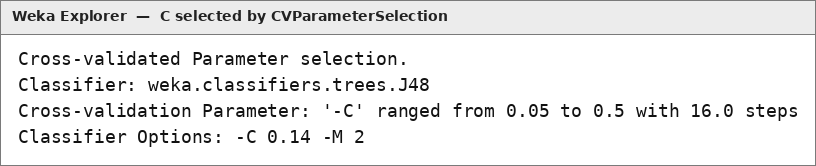
\includegraphics[width=\textwidth]{figures/q4c-selected-c.png}
\caption{Parameter chosen on the full training set. The line \texttt{Classifier Options: -C 0.14 -M 2} is the selected setting.}
\end{figure}

\textbf{Selected value.} The confidence factor selected by CVParameterSelection is $C=0.14$.

%----------------------------------------------------------------------
\section{Question 5: Classification in Python}

The program is \texttt{src/q5\_abalone.py}. It reads \texttt{abalone.data} with no header. The columns in file order are Sex, Length, Diameter, Height, Whole weight, Shucked weight, Viscera weight, Shell weight, and Rings. The new table keeps Length, Diameter, Height, and Whole weight, and sets
\[
\mathrm{Mature}=\begin{cases}1 & \text{if Rings}>8,\\ 0 & \text{otherwise.}\end{cases}
\]
The first three raw ring counts are 15, 7, and 9, so the first three labels are 1, 0, and 1. The 8:2 split is \texttt{train\_test\_split} with \texttt{test\_size=0.2} and \texttt{random\_state=42} (3{,}341 training rows and 836 test rows; $3341+836=4177$). Grid search uses only the training rows, \texttt{DecisionTreeClassifier}, scoring \texttt{f1} (binary F1 for the positive label 1), and the default 5-fold cross-validation. The grid is \texttt{criterion} $\in\{\mathrm{gini},\mathrm{entropy}\}$ and \texttt{max\_depth} $\in\{3,\ldots,10\}$.

\subsection*{5(a) Step 1}

\lstinputlisting[firstline=8,lastline=46,firstnumber=8]{../src/q5_abalone.py}

\begin{figure}[H]
\centering
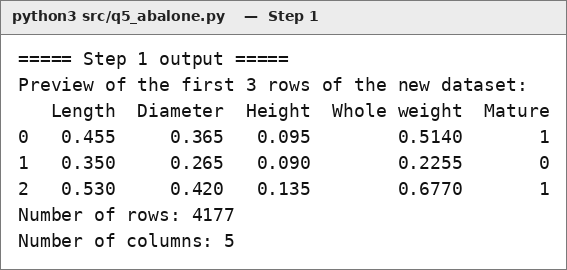
\includegraphics[width=0.92\textwidth]{figures/q5-step1.png}
\caption{Step 1 output: the first three rows of the new dataset, and its shape $4177\times 5$.}
\end{figure}

\subsection*{5(b) Steps 2 and 3}

\lstinputlisting[firstline=49,lastline=79,firstnumber=49]{../src/q5_abalone.py}

\begin{figure}[H]
\centering
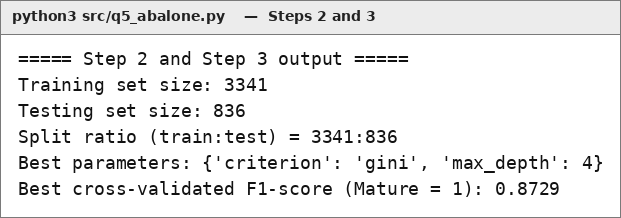
\includegraphics[width=0.95\textwidth]{figures/q5-step23.png}
\caption{Steps 2 and 3 output. The selected parameters are \texttt{criterion=gini} and \texttt{max\_depth=4}. The best cross-validated F1-score for Mature $=1$ is $0.8729$.}
\end{figure}

\subsection*{5(c) Step 4}

\lstinputlisting[firstline=82,lastline=91,firstnumber=82]{../src/q5_abalone.py}

\begin{figure}[H]
\centering
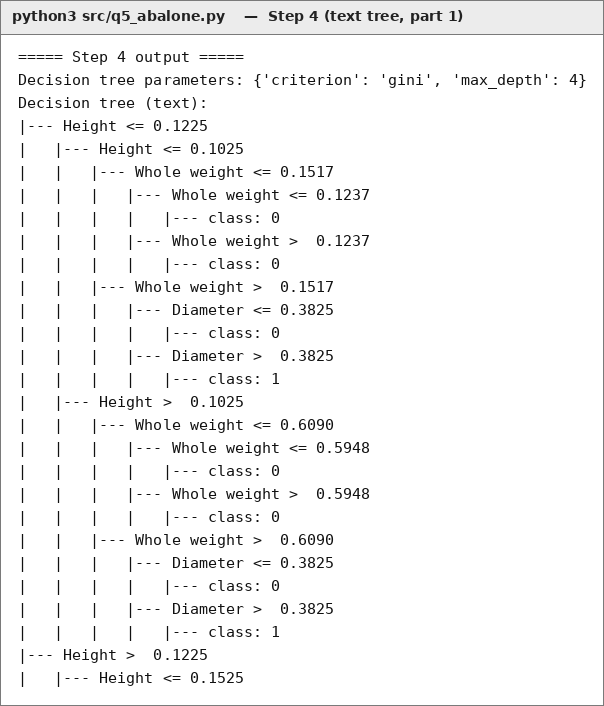
\includegraphics[width=0.78\textwidth]{figures/q5-step4a.png}
\caption{Step 4 output, first part of the text tree. The fitted parameters are gini and max depth 4.}
\end{figure}

\begin{figure}[H]
\centering
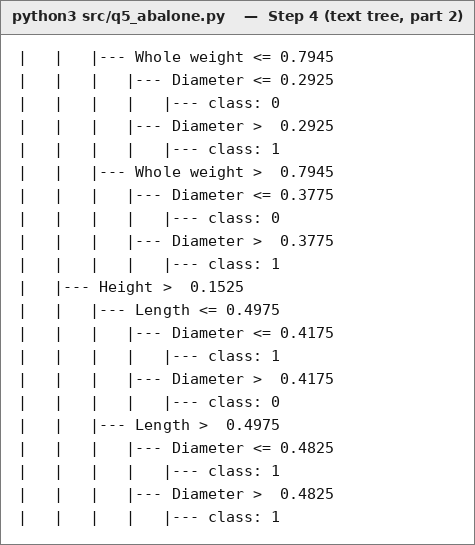
\includegraphics[width=0.72\textwidth]{figures/q5-step4b.png}
\caption{Step 4 output, remainder of the same text tree.}
\end{figure}

\subsection*{5(d) Step 5}

\lstinputlisting[firstline=94,lastline=106,firstnumber=94]{../src/q5_abalone.py}

\begin{figure}[H]
\centering
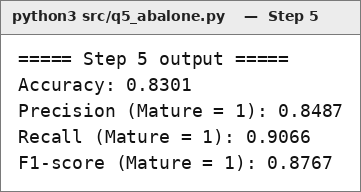
\includegraphics[width=0.78\textwidth]{figures/q5-step5.png}
\caption{Step 5 output on the held-out 20\%, scored for class Mature $=1$.}
\end{figure}

\noindent
On the test set the decision tree has accuracy $0.8301$, precision $0.8487$, recall $0.9066$, and F1-score $0.8767$, all for Mature $=1$ except accuracy, which is the overall accuracy.

\end{document}
